% Template LaTeX file for MInfSem papers
%
% To generate the correct references using BibTeX, run
%     latex, bibtex, latex, latex
% modified...
% - from DAFx-00 to DAFx-02 by Florian Keiler, 2002-07-08
% - from DAFx-02 to DAFx-03 by Gianpaolo Evangelista
% - from DAFx-05 to DAFx-06 by Vincent Verfaille, 2006-02-05
% - from DAFx-06 to DAFx-07 by Vincent Verfaille, 2007-01-05
%                          and Sylvain Marchand, 2007-01-31
% - from DAFx-07 to DAFx-08 by Henri Penttinen, 2007-12-12
%                          and Jyri Pakarinen 2008-01-28
% - from DAFx-08 to DAFx-09 by Giorgio Prandi, Fabio Antonacci 2008-10-03
% - from DAFx-09 to DAFx-10 by Hannes Pomberger 2010-02-01
% - from DAFx-10 to DAFx-12 by Jez Wells 2011
% - from DAFx-12 to DAFx-14 by Sascha Disch 2013
% - from DAFx-14 to MInfSem by Wolfgang Fohl 2014
%
% Template with hyper-references (links) active after conversion to pdf
% (with the distiller) or if compiled with pdflatex.
%
% 20060205: added package 'hypcap' to correct hyperlinks to figures and tables
%                      use of \papertitle and \paperauthorA, etc for same title in PDF and Metadata
%
% 1) Please compile using latex or pdflatex.
% 2) If using pdflatex, you need your figures in a file format other than eps! e.g. png or jpg is working
% 3) Please use "paperftitle" and "pdfauthor" definitions below

%------------------------------------------------------------------------------------------
%  !  !  !  !  !  !  !  !  !  !  !  ! user defined variables  !  !  !  !  !  !  !  !  !  !  !  !  !  !
% Please use these commands to define title and author of the paper:
\def\papertitle{Herausforderungen bei open source Intelligence (OSINT)}
\def\paperauthorA{Lennart Karsten}


%------------------------------------------------------------------------------------------
\documentclass[twoside,a4paper]{article}
\usepackage{minfsem}
\usepackage{amsmath,amssymb,amsfonts,amsthm}
\usepackage{euscript}
\usepackage[utf8]{inputenc}
\usepackage[T1]{fontenc}
\usepackage{ifpdf}
\usepackage[ngerman]{babel}
\usepackage[babel,german=quotes]{csquotes} % Für gute Anführungszeichen
\usepackage{caption}
\usepackage{subfig, color}

\setcounter{page}{1}
\ninept

\usepackage{times}
% Saves a lot of ouptut space in PDF... after conversion with the distiller
% Delete if you cannot get PS fonts working on your system.

% pdf-tex settings: detect automatically if run by latex or pdflatex
\newif\ifpdf
\ifx\pdfoutput\relax
\else
   \ifcase\pdfoutput
      \pdffalse
   \else
      \pdftrue
\fi

\ifpdf % compiling with pdflatex
  \usepackage[pdftex,
    pdftitle={\papertitle},
    pdfauthor={\paperauthorA},
    colorlinks=false, % links are activated as colror boxes instead of color text
    bookmarksnumbered, % use section numbers with bookmarks
    pdfstartview=XYZ % start with zoom=100% instead of full screen; especially useful if working with a big screen :-)
  ]{hyperref}
  \pdfcompresslevel=9
  \usepackage[pdftex]{graphicx}
  \usepackage[figure,table]{hypcap}
\else % compiling with latex
  \usepackage[dvips]{epsfig,graphicx}
  \usepackage[dvips,
    colorlinks=false, % no color links
    bookmarksnumbered, % use section numbers with bookmarks
    pdfstartview=XYZ % start with zoom=100% instead of full screen
  ]{hyperref}
  % hyperrefs are active in the pdf file after conversion
  \usepackage[figure,table]{hypcap}
\fi

\title{\papertitle}

%--------------AUTHOR HEADER STARTS -----------------------
\affiliation{
\paperauthorA,}% \sthanks{This work was supported by the XYZ Foundation}}
{\href{http://www.haw-hamburg.de/ti-i}{Hamburg University of Applied Sciences,
    Dept. Computer Science,} \\ Berliner Tor 7\\ 20099 Hamburg, Germany\\
{\ttfamily \href{mailto:your.name@haw-hamburg.de}{lennart.karsten@haw-hamburg.de}}
}
%-----------------------------------AUTHOR HEADER ENDS------------------------------------------------------

\begin{document}
% more pdf-tex settings:
\ifpdf % used graphic file format for pdflatex
  \DeclareGraphicsExtensions{.png,.jpg,.pdf}
\else  % used graphic file format for latex
  \DeclareGraphicsExtensions{.eps}
\fi

\maketitle

\begin{abstract}
Durch den massiven Anstieg in der Nutzung von Social Media Plattformen, wie Twitter oder Facebook, hat dessen Wichtigkeit für die Gewinnung von \textit{Business intelligence} Informationen in den vergangenen Jahren stark zugenommen. \\
Die Erhebung von Daten aus solchen, meist frei zugänglichen Quellen ist deutlich kostengünstiger als die Erhebung aus klassischen Quellen. Dies hat dazu geführt, dass Open Source Intelligence (OSINT) mittlerweile die wichtigste Quelle zu Gewinnung von \textit{Business intelligence} ist.\\
Im Gegensatz zu klassischen Aggregierungsmethoden ist die Beschaffung einer ausreichenden Menge an Daten beim OSINT kein Problem. Probleme Ergeben sich durch große Mengen an Daten, die teilweise widersprüchlich oder falsch sein können. \\
Die Ausarbeitung befasst sich mit der Beschreibung solcher Problemstellungen und nennt verschiedene Lösungsansätze.
\end{abstract}


\section{Einleitung}
Das Finden von Informationen zur Entscheidungsfindung war noch bis vor ein paar Jahren eine aufwendige Aufgabe. Um ein umfassendes Bild über eine Personengruppe oder eine einzelne Person zu erlangen mussten eine Vielzahl von Quellen ausgewertet werden. Der Vorgang war zeitintensiv und somit teuer.\\
Durch die alltäglichen Nutzung des Internets durch Millionen von Personen hat sich das Bild gewandelt. Es ist mittlerweile möglich Daten massenhaft zu speichern und auszuwerten. Die Qualität der gesammelten Daten hat mit dieser neuen Methode jedoch massiv abgenommen. Dies ergibt sich daraus, dass jeder Benutzer beliebige Daten im Netz über sich streuen kann. Um Die Daten auswerten zu können müssen diese vergleichbar gemacht werden. Außerdem muss bedacht werden, dass Ergebnisse aus einer derartigen elektronischen Auswertung niemals zu 100\% korrekt sein können.

\section{Vergleichbare Arbeiten}
\cite{challanges_in_osint}
\enquote{Challenges in Open Source Intelligence}\\
Beschreibt allgemeine Schwierigkeiten bei OSINT. Der Schwerpunkt liegt bei dieser Arbeit auf der Filterung von erhobenen Daten um diese nutzbar zu machen.\vspace{2mm}

\noindent\cite{challenges_to_automated_alloegory}
\enquote{Challenges to Automated Allegory Resolution in Open Source Intelligence}\\
Die Arbeit befasst sich insbesondere mit Problemen bei der Auswertung von Sprache an konkreten Beispielen.\vspace{2mm}

\noindent\cite{development_of_a_hybrid_decision_system}
\enquote{Development of a Hybrid Decision Support System for intelligence analysis}\\
Im Gegensatz zu den übrigen Arbeiten befasst diese sich nicht mit dem Versuch Analyse nach Möglichkeit zu automatisieren. Stattdessen wird OSINT als Werkzeug, welches dem Analysten Hilfestellungen liefert begriffen. \vspace{2mm}

\noindent\cite{data_consolidation_solution}
\enquote{Data consolidation solution for internal security needs}\\
In der Arbeit wird der Einsatz in Indien beschrieben. Der Fokus liegt in dem Versuch alltägliche Abläufe in der Gesellschaft zu optimieren.


\section{Datensammlung}
Das Sammeln von Daten für die Durchführung von OSINT unterscheidet sich maßgeblich im Vergleich zu klassischen Verfahren. Der folgenden Abschnitte beleuchten diese Unterschiede, da sie für die Art der Nutzung von Bedeutung sind.

\subsection{klassische Datensammlung}
Bei der klassische Gewinnung von Daten wird die Erhebung manuell durchgeführt. Es ist somit möglich, beliebige Quellen zu nutzen, z.B. Zeitungsartikel, handschriftliche Notizen, Tonaufnahmen oder mündliche Aussagen von Personen.\\
Die klassische Datensammlung geschieht mit dem Ziel, bestimmte Informationen heraus zu finden oder einen sehr speziellen Themenkomplex zu erschließen. Für diese Art der Datensammlung können jegliche Art von Daten genutzt werden, da eine manuelle Zusammenführung von Personen getätigt wird.

\subsection{automatisierte Datensammlung}
Beim OSINT werden die Daten zum größten Teil maschinell ausgewertet. Möglich ist eine solche Auswertung durch die gesellschaftlichen Veränderungen, die uns das WEB 2.0 gebracht hat. \\
Seit ein paar Jahren kommunizieren wir mit zunehmendem Maße schriftlich, digital und häufig öffentlich. 
OSINT macht sich diese Tatsache zu Nutzen. Es erfasst und wertet Daten aus Social Media Plattformen wie Twitter, Facebook und Blogs und anderen frei zugänglichen Quellen aus.\\
Da dies Auswertung automatisiert vorgenommen wird, ist die Verarbeitung von großen Mengen an Daten möglich.
 
\subsection{Vergleich}
Wie aus Tabelle~\ref{tab:Vergleich} zu ersehen ist, eignet sich OSINT insbesondere dann, wenn viele Daten betroffen sind und keine hohe Korrektheit der Daten von Nöten ist.

\begin{table}[htdp]
  \caption{\it Vergleich von klassischer und digitaler Informationsgewinnung mittels OSINT}
  \begin{center}
    \begin{tabular}{|c|c|c|}\hline
      Bereich & klassisch & OSINT \\\hline
      Aufwand der Erhebung (einmalig)	& höher & niedriger\\
      Skalierbarkeit der Erhebung 		& schlechter & besser\\
      Aufwand der Auswertung (einmalig) 	& hoch & hoch\\
	  Skalierbarkeit der Auswertung 		& schlechter & besser\\
	  Qualität der Auswertung 			& höher & niedriger\\	  
     \hline
    \end{tabular}
  \end{center}
  \label{tab:Vergleich}
\end{table}


\section{Datenbereinigung}
Gesammelte OSINT Daten enthalten eine Vielzahl von Fehlern. Hierzu gehören: Unterschiedliche Schreibweise von Wörtern, Dopplungen, sowie Widersprüche. Nach  \cite{data_consolidation_solution} gibt es die folgenden Phasen.

\subsection{Untersuchung}
In dieser Phase werden allgemeine Fehler auf Basis von Querreferenzierung und Plausibilitätsüberprüfung gefunden und entfernt. \\
\textbf{Bsp}. \{Teststrasse, Test Straße, Teststr.\} -> \{Teststrasse, Teststrasse, Teststrasse\}

\subsection{Standardisierung}
\label{sub:Standardisierung}
Anschließend werden die Daten in ein einheitliches Format gebracht um sie effizient durchsuchen zu können. Zudem werden Rechtschreibfehler korrigiert. \\
\textbf{Bsp}.: \{Teststrasse, Teststrasse, Teststrasse\} -> \{Teststraße, Teststraße, Teststraße\}.

\subsection{Beseitigung von Dopplungen}
\label{sub:Dopplungen}
In der 3. Phase werden redundante Daten entfernt. Hierbei werden ähnliche Daten zunächst in einem Block zusammengefasst, wodurch die Effizienz der Abgleichung erheblich erhöht werden kann. Im 2. Schritt werden identische Daten pro Block zusammengefasst.\\
\textbf{Bsp}.: \{Teststraße, Teststraße, Teststraße\} -> Teststraße

\subsection{Domain Phase}
Im letzten Schritt werden die gesammelten Daten auf Basis von Domainwissen gefiltert und Themenbereichen zugewiesen. Dies wird im folgenden Abschnitt näher beschrieben.


\section{Zuordnung der OSINT Daten}
Die gesammelten OSINT Daten wurden bereinigt und normalisiert. Um sie effizient nutzen zu können ist es notwendig eine Zuordnung durchzuführen. Dies geschieht auf verschiedenen Ebenen.

\subsection{Thema}
Bedeutungen von Aussagen können in Bezug auf den Kontext in dem sie verwendet werden variieren. Um eine korrekte Aussage über die Bedeutung einer Aussage, oder eines Textes zu treffen, ist es somit notwendig, den Kontext zu bestimmen.\\
Bei vielen Themengebieten ist es zudem von Nöten, eine sprachabhängige Zuordnung durchzuführen. Dies ist notwendig, da in verschiedenen Ländern zu einem Themenkomplex ein anderer \enquote{Major consensus narrative}\footnotemark vorherrschen kann.\\
\noindent Eine thematische Zuordnung kann durch den Einsatz von mehrsprachigen Stichwortlisten geschehen. Bei diesem Ansatz hat jedes bekannte Themengebiet Stichworte, die in einer bestimmten Reihenfolge zu einem gewichteten Ergebnis führen. Hierdurch wird die Wahrscheinlichkeit gemessen, zu der ein Text zu einem Thema gehört.\\
Alternativ gibt es die Möglichkeit die Themenzugehörigkeit mit Hilfe von linearer Algebra zu ermitteln.

\footnotetext{Dieser wird von Bruce Sterling \cite{sterling2001zeitgeist} als das beschrieben, was eine Personengruppe über ein Thema als wahr annimmt. Diese Wahrheit basiert auf dem erlebten und muss nicht zwangsläufig mit den Fakten übereinstimmen.\\
Bsp.: Die gegenläufige Wahrnehmung Europas und Russlands zu dem Krieg in der Ukraine}

\subsection{Geografische Position}
Um eine bessere Thematische Zuordnung durchführen zu können, ist es hilfreich den Aufenthaltsort des Verfassers einer Nachricht zu ermitteln. Dies ist allerdings weniger trivial, als man zunächst annehmen würde.\\
\noindent Ein Grund hierfür ist, dass Orte häufig abgekürzt werden, oder unterschiedliche Schreibweisen haben. Hamburg kann z.B. HH abgekürzt werden und München wird im englischen \enquote{Munich} geschrieben. Orte müssen daher, wie in \ref{sub:Standardisierung} beschrieben, mit Hilfe einer Fuzzysuche angeglichen werden.\\
Erschwerend kommt hinzu, dass ein genannter Ort nicht zwangsläufig der Aufenthaltsort des Verfassers sein muss. In einigen Fällen kann der Aufenthaltsort aus Zusatzdaten ausgelesen werden. Dies könnte beispielsweise eine Twitter Nachricht mit Bild, das eine Georeferenzierung beinhaltet sein.\\
Wenn keine derartige Datenquelle verfügbar ist, muss der Aufenthaltsort aus dem Kontext gelesen werden. Dies erfordert jedoch abhängig von dem Thema ein entsprechend gute thematische Kenntnis. Verbessert werden kann eine derartige geografische Positionsbestimmung bei vielen Nachrichten zum gleichen Thema. 

\subsection{Namen (Named Entity Recognition (NER))}
Um Texte und Aussagen einer Person zuordnen zu können ist es notwendig Namen in Texten zu erkennen und diese als Identität wieder zu erkennen. Dies wird \enquote{Named Entity Recognition (NER)} genannt. Bei der NER gibt es zwei wesentliche Vorgehensweisen. \\
Einerseits ist es Möglich Namen anhand von bestehenden Listen zu erkennen und zuzuordnen.\\
Die andere Möglichkeit ist, Namen anhand von Mustern auszumachen. Z.B. [Anrede] [groß geschrieben] [groß geschrieben] oder [Title] von [Ort]. Bei diesem vorgehen kann eine ungefähre Genauigkeit von 80 Prozent \cite{challanges_in_osint} erreicht werden. Sprachen, die abgesehen von Eigennamen alles klein schreiben wie z.B. Englisch erreichen die besten Erkennungsraten. Sprachen, die Nomen groß schreiben, wie es im Deutschen der Fall ist, erreichen entsprechend schlechtere Ergebnisse. Probleme gibt es bei Sprachen, die keine lateinischen Zeichen verwenden (z.B.: russisch oder chinesisch) und Sprachen, in denen Namen nicht in den Kategorien Vorname und Nachname ausgedrückt werden.

\subsection{Beziehungen}
Beziehungen werden in den Kategorien quantitativ und qualifiziert angegeben.\\
quantitative Beziehung sagen aus, wer wen kennt (Bsp. A kennt B). Eine qualitative Aussage über eine Beziehung zu geben ist relativ einfach. Es bedarf jedoch einer umfangreichen Datenmenge und Zusatzinformationen zu den betroffenen Personen um einen Informationsgewinn zu liefern. Wenn diese Voraussetzungen erfüllt sind, entsteht ein Beziehungskonstrukt. Dieses erlaubt Schlüsse darüber, in welchen Kreisen sich eine Person bewegt.\\
Die qualifizierte Beziehung beschreibt die Art und Intensität des Verhältnisses von Personen (Bsp. A ist verheiratet mit B; A ist befreundet mit C). Ähnlich wie bei der Georeferenzierung ist es bei den qualifizierten Beziehungen schwierig korrekte Informationen zu erlangen. \\
Dies liegt zum einen daran, dass die Daten nur mit einer umfangreichen Textanalyse durchgeführt werden können. Dessen Komplexität steigt mit der Detailtiefe der Beziehung. So wird A B niemals mit "hallo meine Ehefrau B" ansprechen. Zur Erlangung derartiger Informationen können Daten wie der gemeinsame Nachname in Kombination mit übereinstimmenden Adressdaten dienen.\\
Ein weiterer Grund für den erschwerten Umgang mit qualifizierten Beziehungsdaten ist, dass sich diese ändern können. Personen, die beispielsweise Arbeitskollegen waren könnten eine Beziehung eingehen, was zu Fehlern bei Auswertungen führt.\\
Eine qualifizierte Beziehungsanalyse erfordert einen größeren Aufwand, liefert jedoch bessere Ergebnisse.\\
Abbildung \ref{img:Beziehungen} ein Beziehungsnetzwerk von weltweiten Führungspositionen. Die Daten wurden aus Nachrichtenberichten ermittelt.

\begin{figure}[h!]
  \centering
    \reflectbox{%
      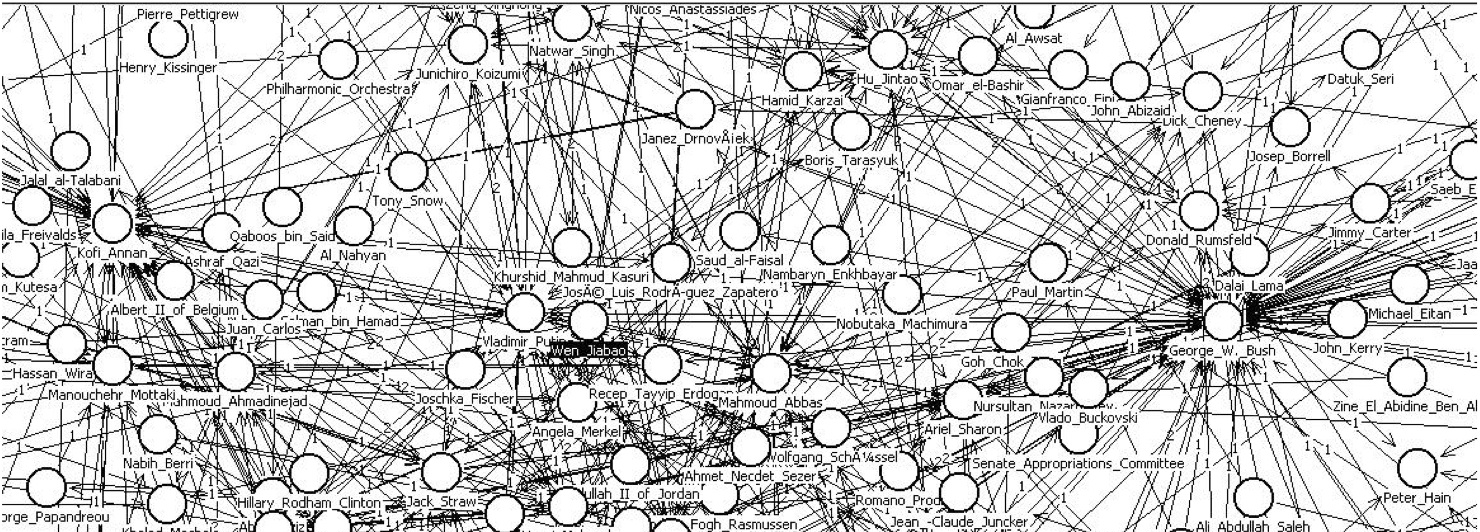
\includegraphics[width=83.5truemm]{img/Beziehungen}}
      %\includegraphics[width=175truemm]{img/beziehungen}}
  \caption{Kommunikationen von Führungspersonen auf Basis von Nachrichten aus dem Jahre 2006. \cite{challanges_in_osint}}
  \label{img:Beziehungen}
\end{figure}

\subsection{Ereignisse}
Um eine Quelle besser nutzen zu können ist es von Vorteil diese einem Ereignis zuordnen zu können. Hierzu ist es wichtig Ereignisse zu erkennen und diese voneinander zu unterscheiden. Ereignisse mit vielen Quellen werden im allgemeinen als wichtig angesehen. Die Erkennung von Dopplungen, wie in Abschnitt \ref{sub:Dopplungen} beschrieben ist hierbei besonders wichtig.\\
Zur Erkennung, ob und wie gut ein Dokument in einen Themenbereich passt werden Texte mit Stichworten versehen. Stichwörter sind Wörter mit dem geringsten Informationsgehalt. Das ganze Dokument wird bei diesem Ansatz als Vektor dargestellt. Jedes Stichwort ist eine Dimension in dem Vektor. Die Werte der Dimension ist die Anzahl, die das Wort vorgekommen ist.\\
Mit dieser Vorgehensweise wird ein Cluster aus Texten erstellt. Das Dokument im Zentrum des Clusters ist das, für das Themengebiet typischste Dokument.


\section{Klassifikatoren}
Die automatisierte Analyse von Texten ist immer Fehlerbehaftet. Die Fehleranfälligkeit variiert mit der Art der Analyse, ebenso wie der Schwellenwert an zulässigen Fehlern.\\
Zur besseren Handhabe mit den verschiedenen Zuständen wurden diese in vier Klassen unterteilt. Diese sind in Tabelle \ref{tab:Klassifikator} dargestellt.

\begin{table}[htdp]
  \caption{\it Klassifikatoren bei der Erkennung}
  \begin{center}
    \begin{tabular}{|c|c|c|}\hline
      					& ist positiv 	& ist negativ \\\hline
       positiv klassifiziert & true positive (TP) & false positive (FP)\\\hline
       negativ klassifiziert & false negativ (FN) & true negative (TN)\\	  
     \hline
    \end{tabular}
  \end{center}
  \label{tab:Klassifikator}
\end{table}

\subsection{Recall (Erinnerung))}
Die Erinnerung gibt den Anteil der positiv Objekte an, die positiv klassifiziert wurden. Die Berechnung lautet:
$$\frac{TP}{(TP+FN)}$$

\subsection{Accuracy (Treffergenauigkeit)}
Die Treffergenauigkeit gibt den Anteil der korrekt Klassifizierten Objekte an. Dieser errechnet sich wie folgt:
$$\frac{TP}{(TP+FP)}$$

\subsection{Precision (Präzision)}
Die Präzision gibt den Anteil der positiv klassifizierten Objekte an, die tatsächlich positiv sind.
$$\frac{(TP+TN)}{(TP+FP+FN+TN)}$$

\section{menschliche Interaktion}
Menschliche Interaktion ist im Gegensatz zur maschinellen Auswertung deutlich kostspieliger und wird deshalb maximal gering gehalten. Abhängig von dem Vorhaben sind jedoch nur gewisse Fehlertoleranzen akzeptabel. Häufig sind besonders FP Ergebnisse ein Problem, da sie zur Verfälschung des Endergebnisses führen.\\
Um dies zu vermeiden wird der Schwellwert der erreicht werden muss um ein Positives Ergebnis zu liefern erhöht. In der Folge steigen dafür die FN Ergebnisse an. Diese sind für eine korrekte Analyse jedoch wenig Problematisch.\\
Zur Verbesserung der Ergebnisse und einer besseren Erkennung werden geschulte Personen eingesetzt. Diese überprüfen Ergebnisdaten auf ihre Korrektheit. Häufige Fehler sind z.B. Ereignisse, die jährlich auftreten und deshalb von dem System als eigenständiges und nicht als sich wiederholendes Ereignis erkannt werden.


\section{Vertrauen und Wahrheit}
Das wahrscheinlich problematischste Feld von OSINT ist das Vertrauen in Aussagen und die Prüfung dessen Wahrheitsgehalt.\\
Bei Kommunikationspartner, die sich gut kennen wird häufig ein Teil der Informationen weg gelassen, da sie beim Kommunikationspartner bekannt sind. Dies tritt insbesondere dann auf, wenn ein Kanalwechsel vollzogen wird. Z.B. wenn eine persönliche Kommunikation auf dem digitalen weg fortgeführt wird.\\
Ein weiteres Problem bei der Validierung von Aussagen sind Übertreibungen. Diese verfälschen Fakten und eine Korrektur ist nur durch den Abgleich mit Referenzquellen möglich.\\
Eine ebenso große Herausforderung stellen Unwahrheiten und Ironie dar. Sie sind für technische Systeme nahezu nicht zu erkennen. Ein Mensch kann mit ausreichendem Hintergrundwissen diese unter Umständen ausgleichen.\\
Ein weiteres Problem sind Vorurteile. Diese sind selbst für erfahrene Analysten ein Problem, da sie das Urteilsvermögen negativ beeinflussen.\\
Um die Wahrheit einer Quelle zu ermitteln kann diese auf Basis ihrer vergangenen Aussagen eingestuft werden. Quellen mit hoher Seriosität bekommen somit eine höhere Gewichtung, sodass das Ergebnis verbessert werden kann.\\
Es ist zudem hilfreich Quellen in Kategorien zu unterteilen um deren Aussagen unter Berücksichtigung verschiedener Faktoren zu beurteilen. Mögliche Typen sind:
\begin{itemize}
	\item unabhängig
	\item Regierung
	\item Rebellen
	\item politisch
	\item usw.
\end{itemize}
Zudem wird häufig dem Bericht ein Typ zugewiesen. Mögliche Typen sind:
\begin{itemize}
	\item erste Hand
	\item vom hören sagen
	\item Meinung
	\item Duplikat
	\item zensiert
	\item usw.
\end{itemize}


\section{OSINT Wissensbasis}
Zur erfolgreichen Durchführung von OSINT bedarf es verschiedener Voraussetzungen. Hierzu zählen unter anderem detaillierte Domain Kenntnisse. Für die automatisierte Analyse ist eine Datenbank mit Metadaten der Domain zu erstellen.\\
Zur effizienten Nutzung ist es wichtig, Frontend Anwendungen bereit zu stellen. Eine dieser Werkzeuge sind:
\begin{itemize}
	\item Netminer \cite{netminer}
	\item Commetrix \cite{commetrix}
	\item Gephi \cite{gephi}
	\item Cyc \cite{cyc}
\end{itemize}

\subsection{Länderprofile}
Viele Vorkommnisse sind länderübergreifend. Um diese effizient analysieren zu können ist es notwendig jedes Land in Bezug zu seinem Kontext zu betrachten. Hierbei muss die politische, sowie die gesellschaftliche Lage eines Landes beachtet werden. Beispielsweise sind schwere Ausschreitungen in einem Land mit stabiler Wirtschaftslage unwahrscheinlicher und damit von größerer Bedeutung als Ausschreitungen in einem Land in schwieriger Lage.\\
Die Faktoren, die eine Land, oder eine Region auszeichnen werden als strukturelle Indikatoren bezeichnet.

\subsection{Strukturelle Indikatoren}
%- quantifiziert sozialpolitische Faktoren
%- basieren auf verschiedenen statistischen Werten
%-- Wirtschaftswachstum
%-- Bildungsgrad
%-- Lebenserwartung
%-- Arbeitslosenquote
%-- usw.
%- werden zu Faktoren, wie der "Lebensqualität" oder "Konfliktkapazität" zusammengefasst.
%- ermöglicht Situationen von Ländern zu vergleichen

Strukturelle Indikatoren sind qualifizierte sozialpolitische Faktoren. Diese basieren auf verschiedenen statistischen Werten. Einige davon sind:
\begin{itemize}
	\item Wirtschaftswachstum
	\item Bildungsgrad
	\item Lebenserwartung
	\item Arbeitslosenquote
\end{itemize}
Um Werte vergleichbar zu halten werden die gleichen Maßstäbe angelegt. So kann zum Beispiel die Pisa Studie \cite{pisa} zum Vergleich des Bildungsgrats europäischer Länder verwendet werden.\\
Die strukturellen Indikatoren werden zu Faktoren, wie Konfliktkapazität oder Lebensqualität zusammengefasst. Dies dient letztendlich als Basis für einen direkten Vergleich.

\subsection{Aufständische und Terroristen}
%- Das Führen von Listen über terroristische Gruppen wird zumeist händisch durchgeführt
%- OSINT kann die Informationsgewinnung durch eine vorfilterung unterstützen.


\subsection{Datenbank mit Tupeln}
%- Liste mit mächtigen Führern und Wirtschaftsbossen
%- hilft bei der Zuordnung von Ereignissen in einem Land

\subsection{Dynamische Indikatoren}
%- Analyse von sich häufig ändernden Daten
%- Bsp.: Opferzahlen im Irak


\section{P: Challenges to Automated Allegory}



\section{Kritik an OSINT}



\section{Zusammenfassung}


%\newpage
\nocite{*}
\bibliographystyle{IEEEbib}
\bibliography{MI-Hausarbeit} % requires file minfsem_tmpl.bib

%\section{Appendix: Margin Check}
%This section shows the column margins for the text. \bigskip\newline

\end{document}
